\documentclass[11pt,compress,t,notes=noshow]{beamer}
\usepackage[]{graphicx}\usepackage[]{color}
% maxwidth is the original width if it is less than linewidth
% otherwise use linewidth (to make sure the graphics do not exceed the margin)
\makeatletter
\def\maxwidth{ %
  \ifdim\Gin@nat@width>\linewidth
    \linewidth
  \else
    \Gin@nat@width
  \fi
}
\makeatother

\definecolor{fgcolor}{rgb}{0.345, 0.345, 0.345}
\newcommand{\hlnum}[1]{\textcolor[rgb]{0.686,0.059,0.569}{#1}}%
\newcommand{\hlstr}[1]{\textcolor[rgb]{0.192,0.494,0.8}{#1}}%
\newcommand{\hlcom}[1]{\textcolor[rgb]{0.678,0.584,0.686}{\textit{#1}}}%
\newcommand{\hlopt}[1]{\textcolor[rgb]{0,0,0}{#1}}%
\newcommand{\hlstd}[1]{\textcolor[rgb]{0.345,0.345,0.345}{#1}}%
\newcommand{\hlkwa}[1]{\textcolor[rgb]{0.161,0.373,0.58}{\textbf{#1}}}%
\newcommand{\hlkwb}[1]{\textcolor[rgb]{0.69,0.353,0.396}{#1}}%
\newcommand{\hlkwc}[1]{\textcolor[rgb]{0.333,0.667,0.333}{#1}}%
\newcommand{\hlkwd}[1]{\textcolor[rgb]{0.737,0.353,0.396}{\textbf{#1}}}%
\let\hlipl\hlkwb

\usepackage{framed}
\makeatletter
\newenvironment{kframe}{%
 \def\at@end@of@kframe{}%
 \ifinner\ifhmode%
  \def\at@end@of@kframe{\end{minipage}}%
  \begin{minipage}{\columnwidth}%
 \fi\fi%
 \def\FrameCommand##1{\hskip\@totalleftmargin \hskip-\fboxsep
 \colorbox{shadecolor}{##1}\hskip-\fboxsep
     % There is no \\@totalrightmargin, so:
     \hskip-\linewidth \hskip-\@totalleftmargin \hskip\columnwidth}%
 \MakeFramed {\advance\hsize-\width
   \@totalleftmargin\z@ \linewidth\hsize
   \@setminipage}}%
 {\par\unskip\endMakeFramed%
 \at@end@of@kframe}
\makeatother

\definecolor{shadecolor}{rgb}{.97, .97, .97}
\definecolor{messagecolor}{rgb}{0, 0, 0}
\definecolor{warningcolor}{rgb}{1, 0, 1}
\definecolor{errorcolor}{rgb}{1, 0, 0}
\newenvironment{knitrout}{}{} % an empty environment to be redefined in TeX

\usepackage{alltt}
\newcommand{\SweaveOpts}[1]{}  % do not interfere with LaTeX
\newcommand{\SweaveInput}[1]{} % because they are not real TeX commands
\newcommand{\Sexpr}[1]{}       % will only be parsed by R



\usepackage[english]{babel}
\usepackage{dsfont}
\newcommand\bmmax{2}
\usepackage{bm}
\usepackage{bbm}
\usepackage{verbatim}
\usepackage{amsmath}
\usepackage{amsfonts}
\usepackage{csquotes}
\usepackage{multirow}
\usepackage{longtable}
\usepackage{enumerate}
\usepackage[absolute,overlay]{textpos}
\usepackage{psfrag}
\usepackage{algorithm}
\usepackage{algorithmicx}
\usepackage{algpseudocode}
\usepackage{eqnarray}
\usepackage{multimedia}
\usepackage{media9}
\usepackage{arydshln}
\usepackage{tabularx}
\usepackage{placeins}
\usepackage{tikz}
\usepackage{setspace}
\usepackage{wrapfig}
\usepackage{tcolorbox}
\usepackage[export]{adjustbox}
\usepackage{siunitx}
\usetikzlibrary{shapes,arrows,automata,positioning,calc}
\def\signed #1{{\leavevmode\unskip\nobreak\hfil\penalty50\hskip1em
  \hbox{}\nobreak\hfill #1%
  \parfillskip=0pt \finalhyphendemerits=0 \endgraf}}

\newsavebox\mybox
\newenvironment{aquote}[1]
  {\savebox\mybox{#1}\begin{quote}\openautoquote\hspace*{-.7ex}}
  {\unskip\closeautoquote\vspace*{1mm}\signed{\usebox\mybox}\end{quote}}
  
\tikzset{
  %Define standard arrow tip
  >=stealth',
  %Define style for boxes
  punkt/.style={
    rectangle,
    rounded corners,
    draw=black, very thick,
    text width=6.5em,
    minimum height=2em,
    text centered},
  % Define arrow style
  pil/.style={
    ->,
    thick,
    shorten <=2pt,
    shorten >=2pt,}
}
\usepackage{subfig}

%new environments

\newenvironment{vbframe}  %frame with breaks and verbatim
{
 \begin{frame}[containsverbatim,allowframebreaks]
}
{
\end{frame}
}

\newenvironment{vframe}  %frame with verbatim without breaks (to avoid numbering one slided frames)
{
 \begin{frame}[containsverbatim]
}
{
\end{frame}
}

\newenvironment{blocki}[1]   % itemize block
{
 \begin{block}{#1}\begin{itemize}
}
{
\end{itemize}\end{block}
}

\newenvironment{fragileframe}[2]{  %fragile frame with framebreaks
\begin{frame}[allowframebreaks, fragile, environment = fragileframe]
\frametitle{#1}
#2}
{\end{frame}}


\newcommand{\myframe}[2]{  %short for frame with framebreaks
\begin{frame}[allowframebreaks]
\frametitle{#1}
#2
\end{frame}}

\newcommand{\remark}[1]{
  \textbf{Remark:} #1
}

%%%%%%%%%%%%%%%%%%%%%%%%%%%%%%%%%%%%%%%%%%%%%%%%%%%%%%%%%%%%%%%%%%%%%%%%%%%%%%%

% basic latex stuff
\newcommand{\pkg}[1]{{\fontseries{b}\selectfont #1}} %fontstyle for R packages
\newcommand{\lz}{\vspace{0.5cm}} %vertical space
\newcommand{\dlz}{\vspace{1cm}} %double vertical space
\newcommand{\oneliner}[1] % Oneliner for important statements
{\begin{block}{}\begin{center}\begin{Large}#1\end{Large}\end{center}\end{block}}


%\usetheme{lmu-lecture}
\usepackage{../style/lmu-lecture}

\let\code=\texttt
\let\proglang=\textsf

\setkeys{Gin}{width=0.9\textwidth}



\title{Introduction to Machine Learning}
\author{Bernd Bischl}
\institute{Department of Statistics -- LMU Munich}
\date{Winter term 2021}

\setbeamertemplate{frametitle}{\expandafter\uppercase\expandafter\insertframetitle}



\begin{document}




\input{../latex-math/basic-math}
\input{../latex-math/basic-ml}
\input{../latex-math/ml-nn}

\lecturechapter{3}{Deep Learning- MLP}
\lecture{Deep Learning- MLP}
%%%%%%%%%%%%%%%%%%%%%%%%%%%%%%%%%%%%%%%%%%%%%%%%%%%%%%%%%%%%%%%%%%

\begin{vbframe}{Motivation}
\lz
\begin{itemize}
\item The graphical way of representing simple functions/models, like logistic regression. Why is that useful?
\lz
\item Because individual neurons can be used as building blocks of more complicated functions.
\lz
\item Networks of neurons can represent extremely complex hypothesis spaces.
\lz
\item Most importantly, it allows us to define the \enquote{right} kinds of hypothesis spaces to learn functions that are more common in our universe in a data-efficient way (see Lin, Tegmark et al. 2016).
\end{itemize}
\framebreak
%%%%%%%%%%%%%%%%%%%%%%%%%%%%%%%%%%%%%%%%%%%%%%%%%%%%%%%%%%%%%%%%%%

\begin{itemize}
\item As a single neuron is restricted to learning only linear decision boundaries, its performance on the following task is quite poor:
\begin{figure}
\centering
\scalebox{0.25}{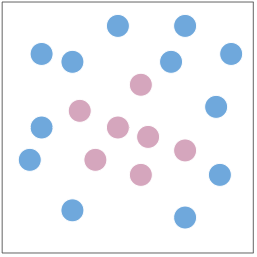
\includegraphics{plots/cartesian.png}}
\end{figure}
\item However, the neuron can easily separate the classes if the original features are transformed (e.g., from Cartesian to polar coordinate): 
\begin{figure}
\centering
\scalebox{0.25}{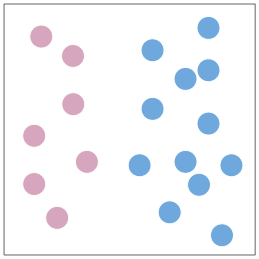
\includegraphics{plots/polar.png}}
\end{figure}
\end{itemize}
\framebreak
%%%%%%%%%%%%%%%%%%%%%%%%%%%%%%%%%%%%%%%%%%%%%%%%%%%%%%%%%%%%%%%%%%

\begin{itemize}
\item Instead of classifying the data in the original representation,
\begin{figure}
\centering
\scalebox{1}{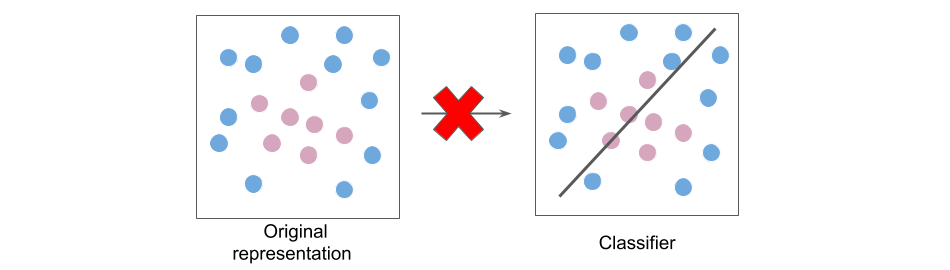
\includegraphics{plots/repold_f.png}}
\end{figure}
\item we classify it in a new feature space.
\begin{figure}
\centering
\scalebox{1}{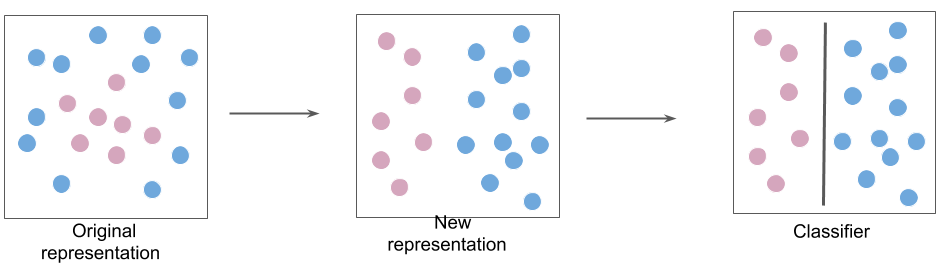
\includegraphics{plots/repnew_f.png}}
\end{figure}
\end{itemize}
\framebreak
%%%%%%%%%%%%%%%%%%%%%%%%%%%%%%%%%%%%%%%%%%%%%%%%%%%%%%%%%%%%%%%%%%
\begin{itemize}
\item Analogously, instead of a single neuron, 
\begin{figure}
\centering
\scalebox{0.6}{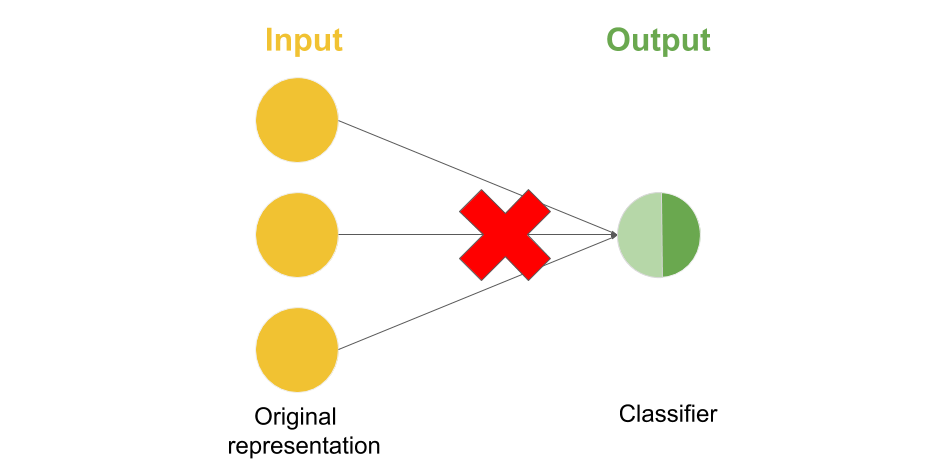
\includegraphics{plots/oldrep_n_f.png}}
\end{figure}
\item we use more complex networks.
\begin{figure}
\centering
\scalebox{0.65}{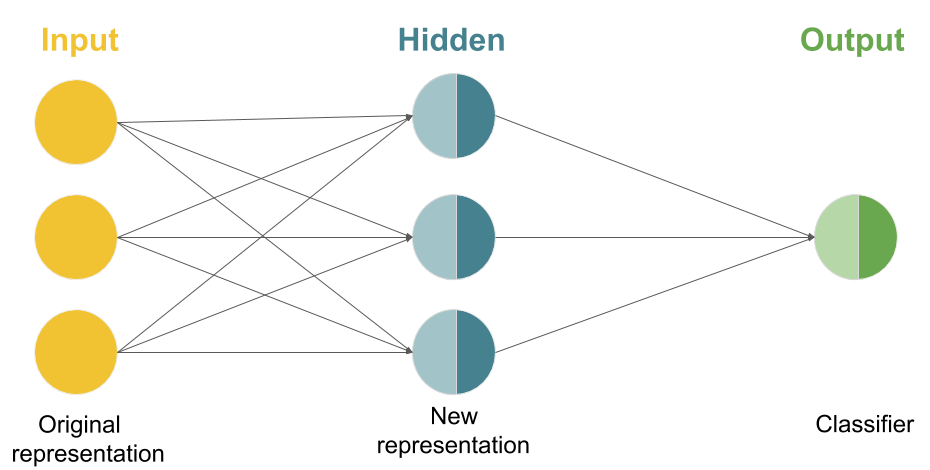
\includegraphics{plots/newrep_n_f.png}}
\end{figure}
\end{itemize}
\end{vbframe}
%%%%%%%%%%%%%%%%%%%%%%%%%%%%%%%%%%%%%%%%%%%%%%%%%%%%%%%%%%%%%%%%%%

\begin{vbframe} {Representation Learning}
  \begin{itemize}
    \vspace{5mm}
    \item It is therefore \textit{very} critical to feed a classifier the \enquote{right} features in order for it to perform well.
    \vspace{7mm}
    \item Before deep learning took off, features for tasks like machine vision and speech recognition were \enquote{hand-designed} by domain experts. This step of the machine learning pipeline is called \textbf{feature engineering}.
    \vspace{7mm}
    \item The single biggest reason DL is so important is that it automates feature engineering. This is called \textbf{representation learning}.
  \end{itemize}
\end{vbframe}
%%%%%%%%%%%%%%%%%%%%%%%%%%%%%%%%%%%%%%%%%%%%%%%%%%%%%%%%%%%%%%%%%%

\begin{vbframe}{Single Hidden Layer Networks}

\textbf{Recall:} a single neuron performs a 2-step computation:
\begin{enumerate}
\item \textbf{Affine Transformation:} weighted sum of inputs plus bias.
\item \textbf{Non-linear Activation:} a non-linear transformation applied to the weighted sum.
\end{enumerate}

\begin{itemize}
\item It is possible to feed multiple inputs to a neural network simultaneously.
\item The inputs $\xi$, for $i \in \nset$, are arranged as rows in the \textbf{design matrix} $\Xmat$.
\item The weighted sum in the hidden layer is now computed as $\Xmat\Wmat + \bm{B}$, where,
\item The \textit{matrix} of hidden activations $\bm{Z} = \sigma(\Xmat\Wmat + \bm{B})$
\item The final output of the network, which contains a prediction for each input, is $\tau(\bm{Z}\wtu + \bm{C})$, where
\end{itemize}
\end{vbframe}
%%%%%%%%%%%%%%%%%%%%%%%%%%%%%%%%%%%%%%%%%%%%%%%%%%%%%%%%%%%%%%%%%%

\begin{frame} {Single Hidden Layer Networks: Example}
  \begin{itemize}
    \item Weights (and biases) of the network.
  \begin{figure}
    \centering
      \only<1>{\scalebox{.8}{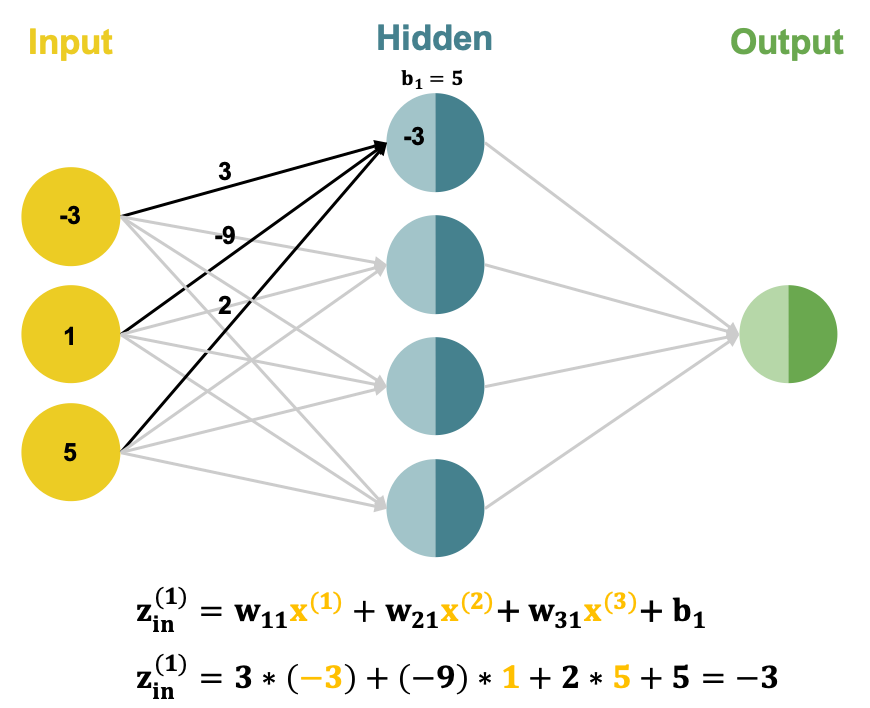
\includegraphics{plots/singlelay_1.png}}}
      \only<2>{\scalebox{.8}{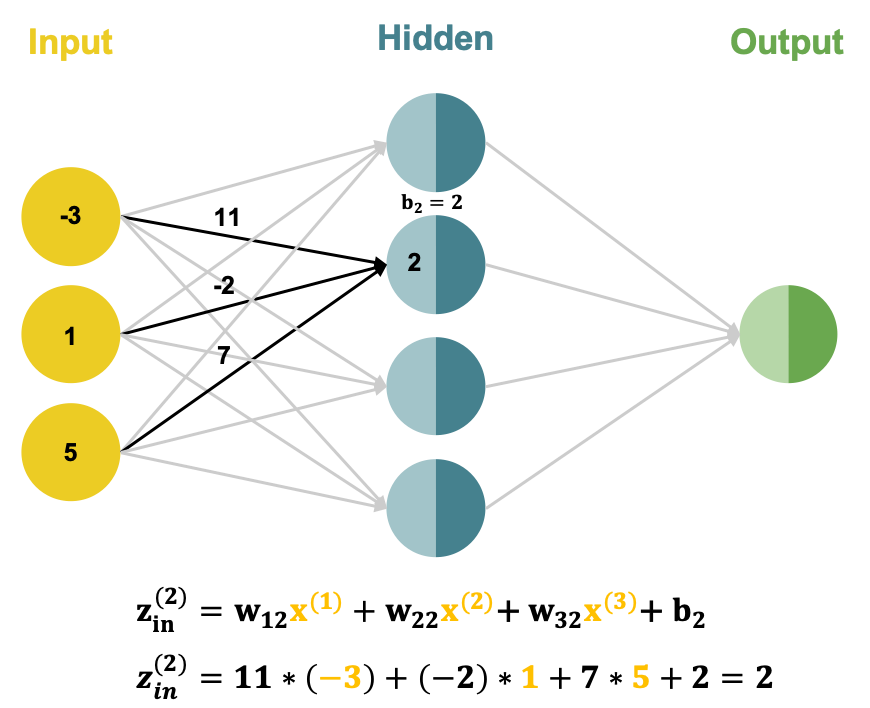
\includegraphics{plots/singlelay_2.png}}}
      \only<3>{\scalebox{.8}{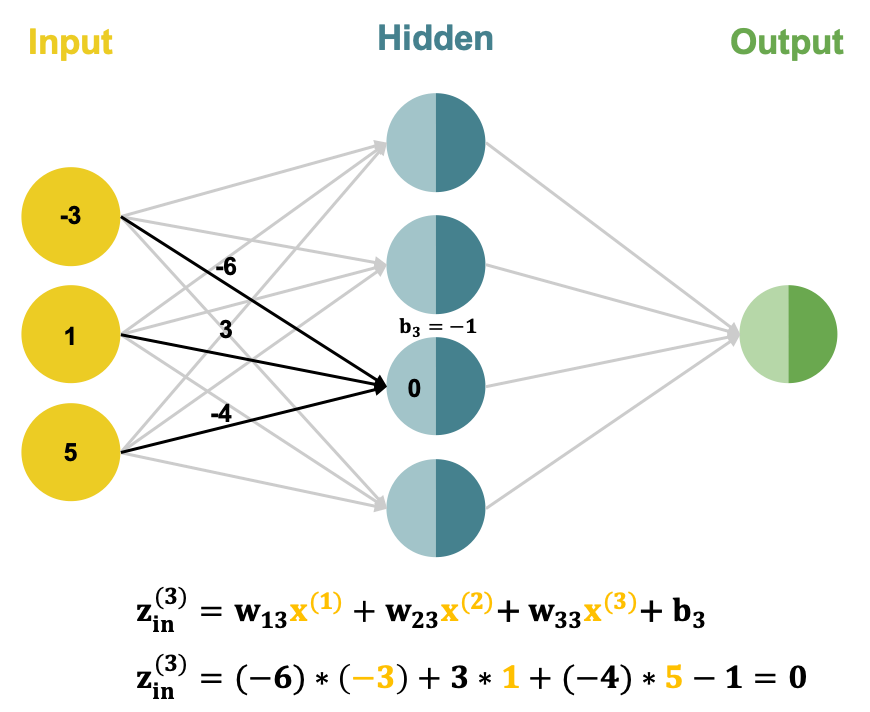
\includegraphics{plots/singlelay_3.png}}}
      \only<4>{\scalebox{.8}{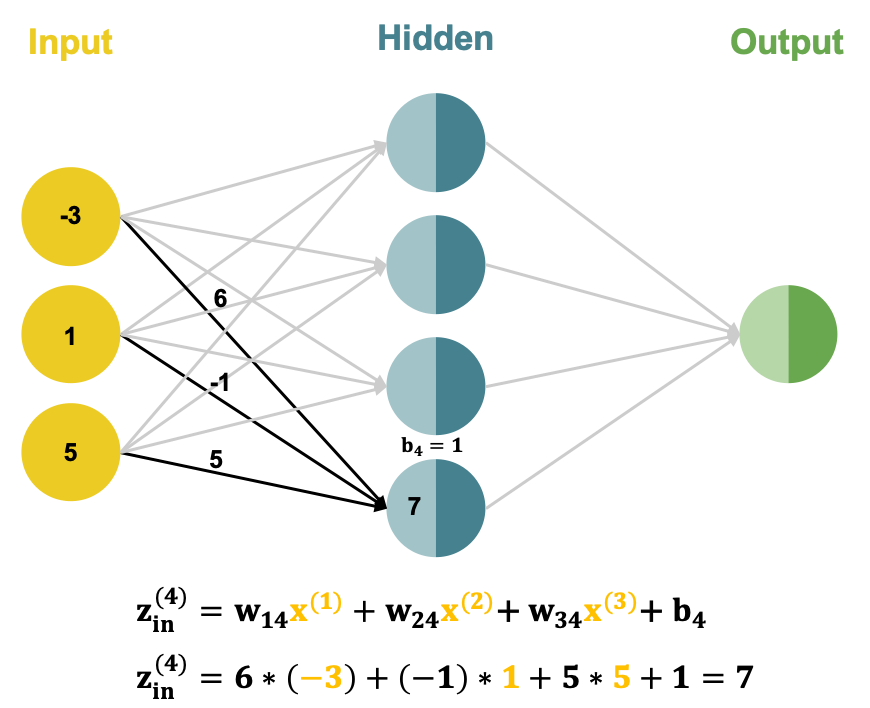
\includegraphics{plots/singlelay_4.png}}}
      \only<5>{\scalebox{.8}{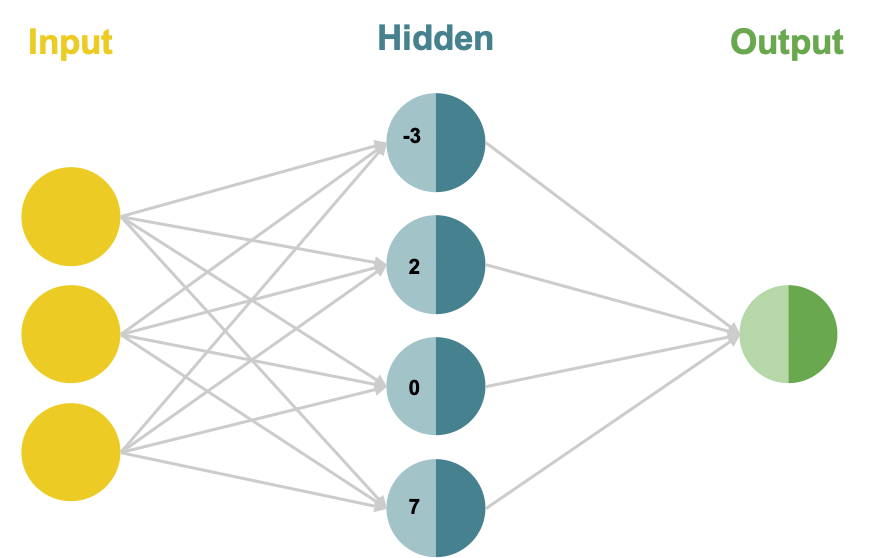
\includegraphics{plots/singlelay_5.png}}}
      \only<6>{\scalebox{.8}{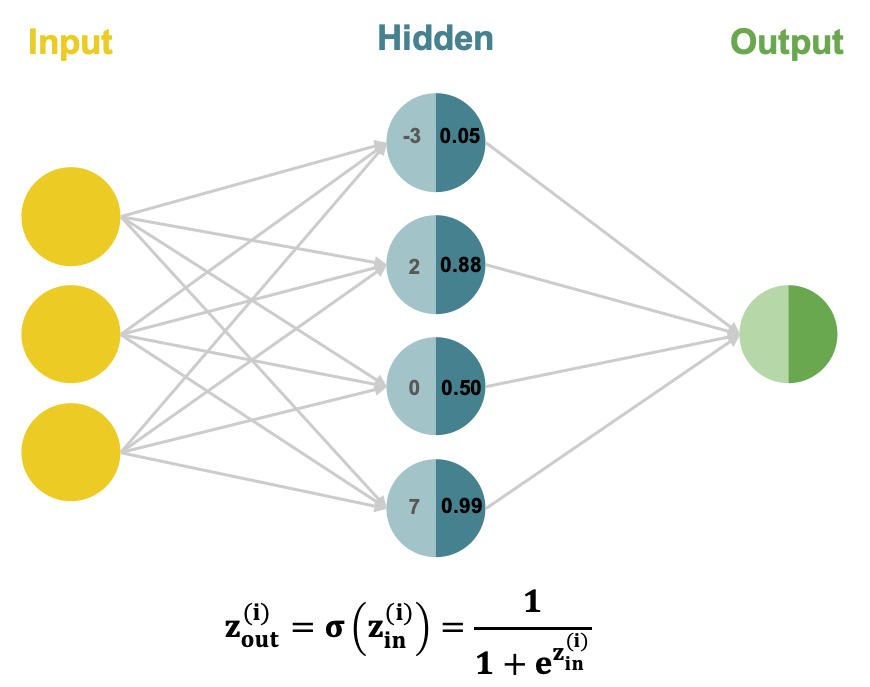
\includegraphics{plots/singlelay_6.png}}}
  \end{figure}
  \begin{figure}
    \centering
  \end{figure}
  \end{itemize}
\end{frame}
%%%%%%%%%%%%%%%%%%%%%%%%%%%%%%%%%%%%%%%%%%%%%%%%%%%%%%%%%%%%%%%%%%

\begin{frame} {Single Hidden Layer Networks: Example}
\small{Forward pass through the shallow neural network.}
  \begin{figure}
    \centering
    \only<1>{\scalebox{.8}{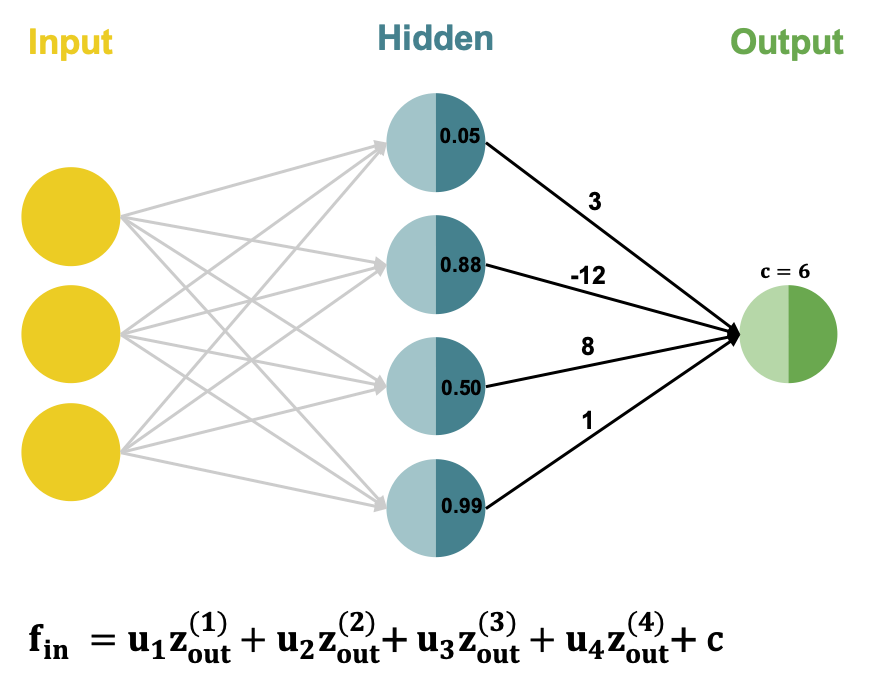
\includegraphics{plots/singlelay_7.png}}}
    \only<2>{\scalebox{.8}{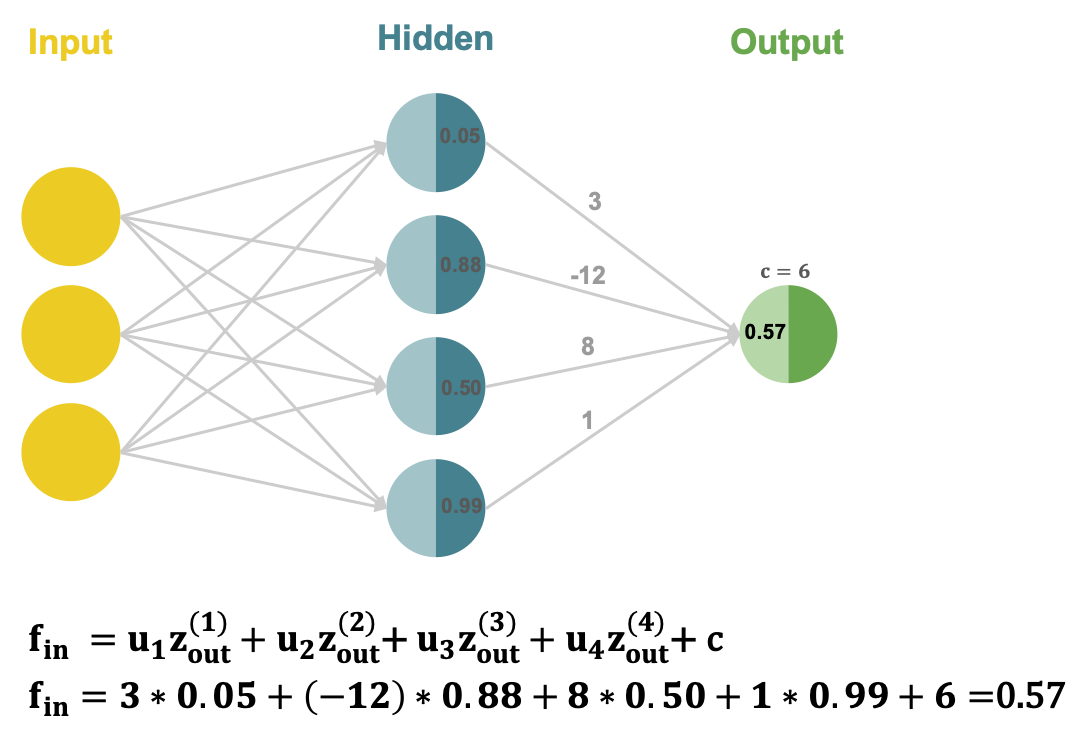
\includegraphics{plots/singlelay_8.png}}}
    \only<3>{\scalebox{.8}{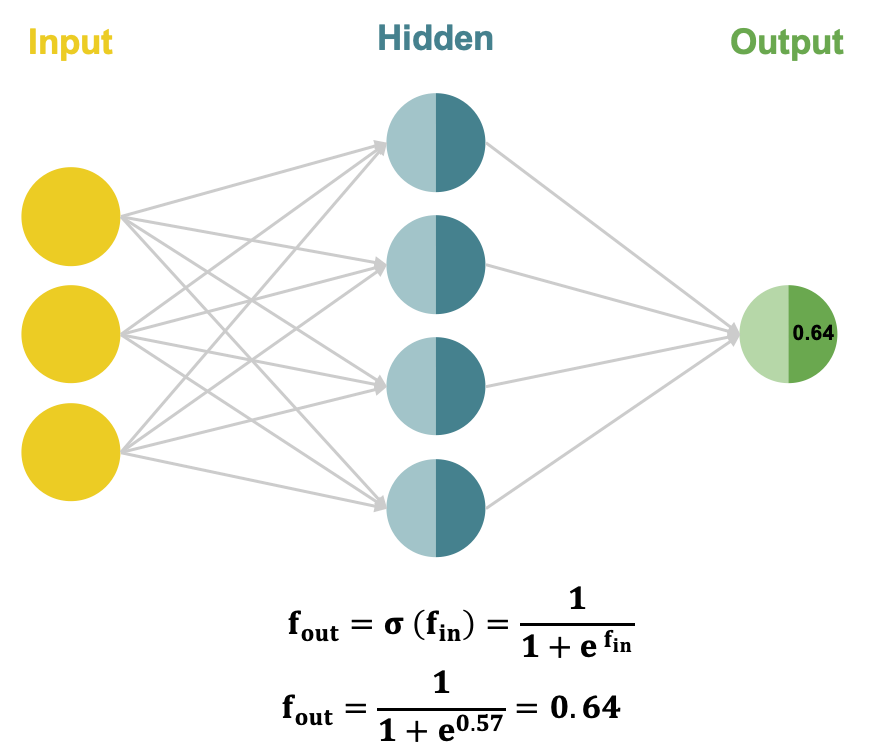
\includegraphics{plots/singlelay_9.png}}}
  \end{figure}
\end{frame}
%%%%%%%%%%%%%%%%%%%%%%%%%%%%%%%%%%%%%%%%%%%%%%%%%%%%%%%%%%%%%%%%%%

\begin{vbframe}{Hidden Layer: Activation Function}
\textbf{Note:} if the hidden layer does not have a non-linear activation, the network can only learn linear decision boundaries.
\begin{blocki}{ReLU Activation:}
\item Currently the most popular choice is the ReLU (rectified linear unit):
$$ \sigma (v) = \max(0,v) $$
\end{blocki}
\begin{figure}
\scalebox{1}{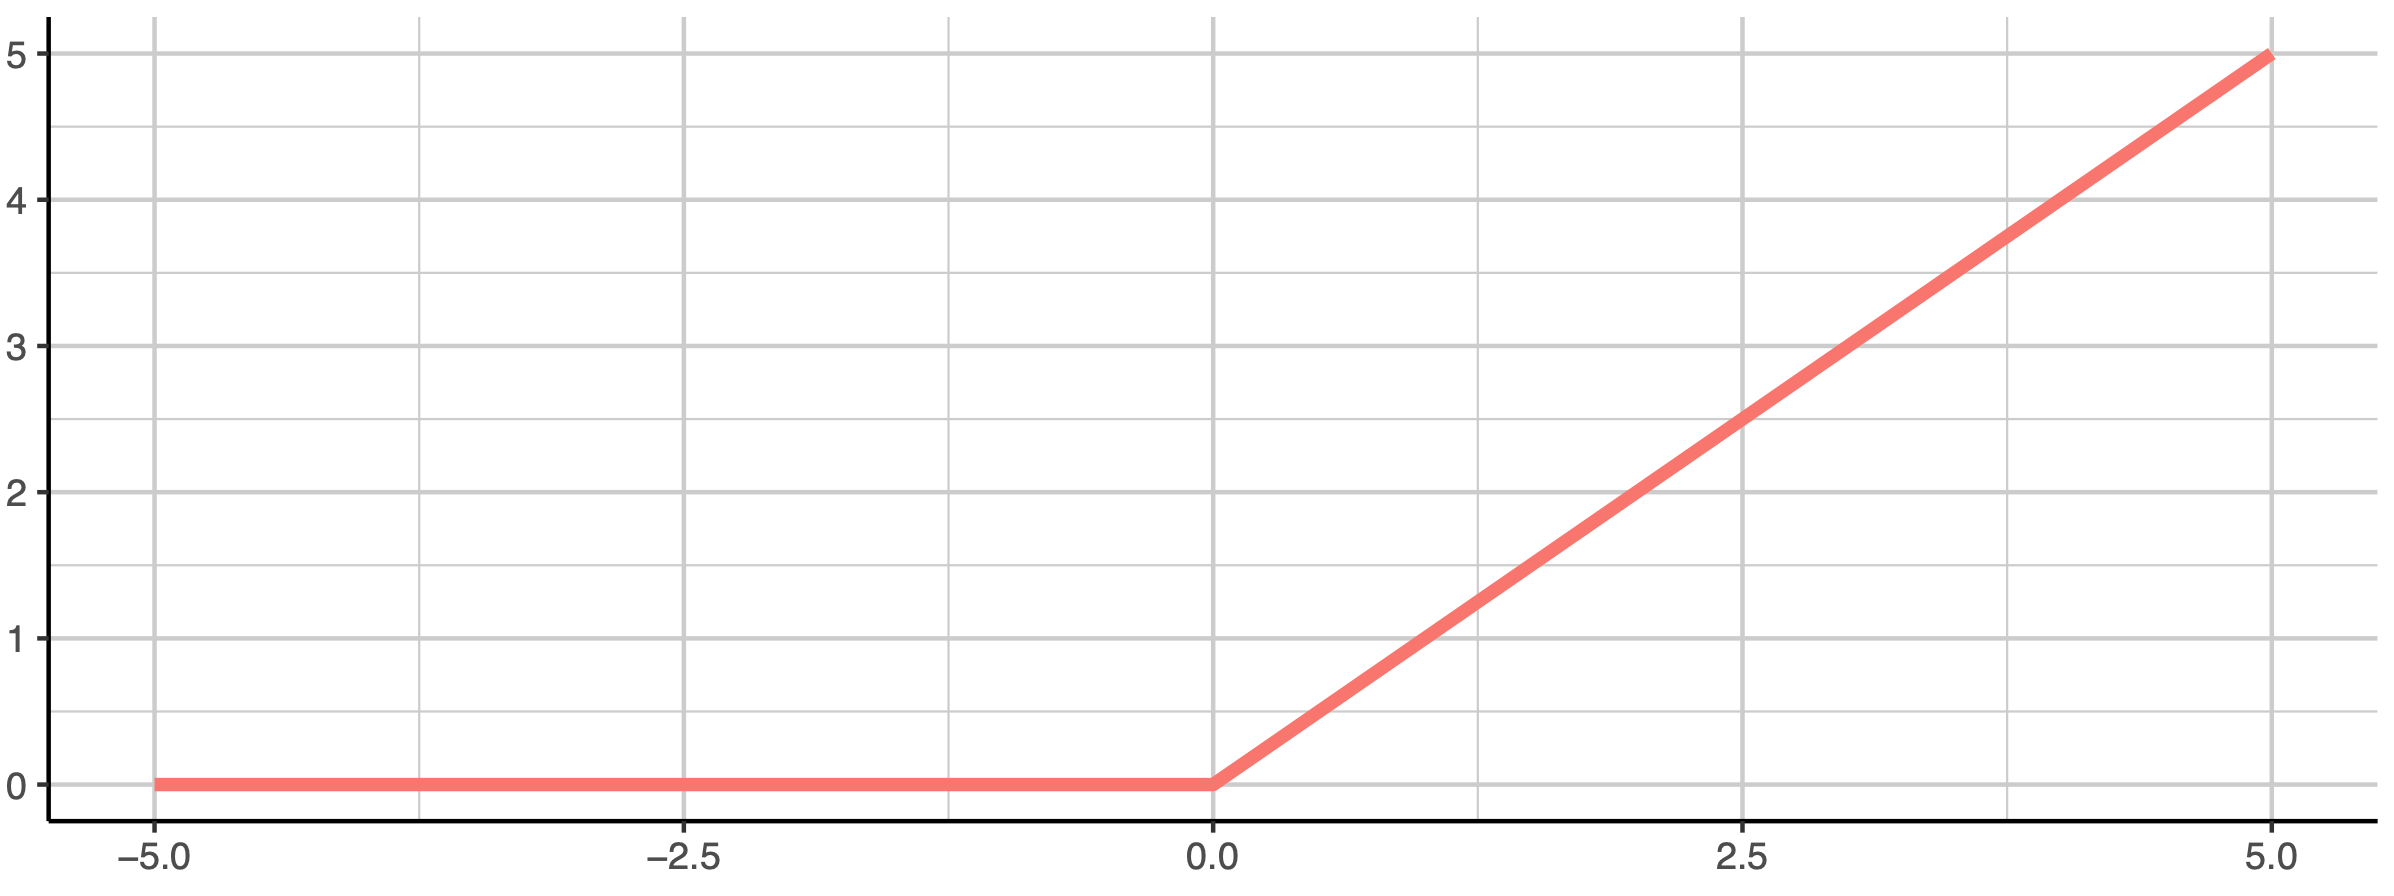
\includegraphics{plots/relu.png}}
\end{figure}
\framebreak
%%%%%%%%%%%%%%%%%%%%%%%%%%%%%%%%%%%%%%%%%%%%%%%%%%%%%%%%%%%%%%%%%%

\begin{blocki}{Hyperbolic Tangent Activation:}
\item Another choice might be the hyperbolic tangent function:
$$ \sigma (v) = \text{tanh}(v) = \frac{\text{sinh}(v)}{\text{cosh}(v)} = 1 - \frac{2}{\exp(2v) + 1}$$
\end{blocki}
\begin{figure}
\scalebox{1}{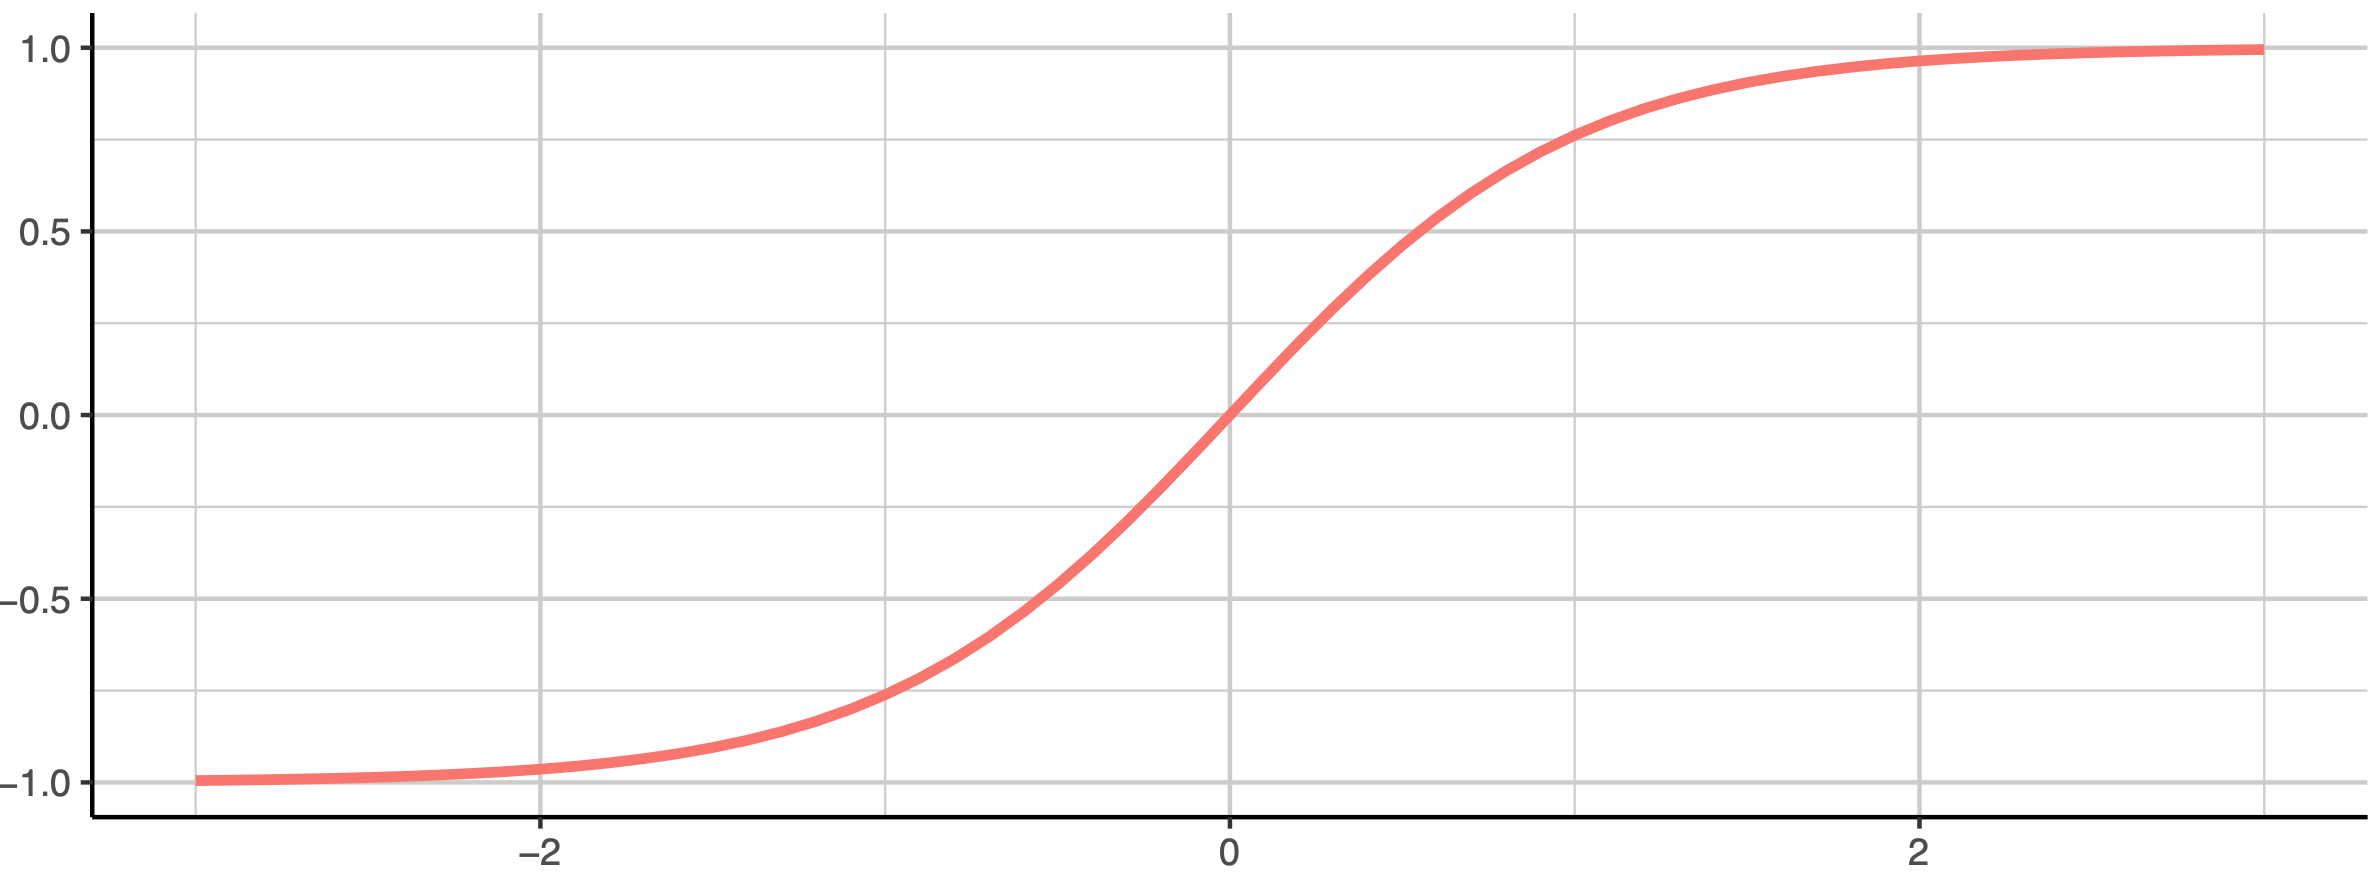
\includegraphics{plots/tanh.png}}
\end{figure}
\framebreak
%%%%%%%%%%%%%%%%%%%%%%%%%%%%%%%%%%%%%%%%%%%%%%%%%%%%%%%%%%%%%%%%%%

\begin{blocki}{Sigmoid Activation Function:}
\item The sigmoid function can be used even in the hidden layer:
$$ \sigma(v) = \frac{1}{1+\exp (-v)} $$
\end{blocki}
\begin{figure}
\scalebox{1}{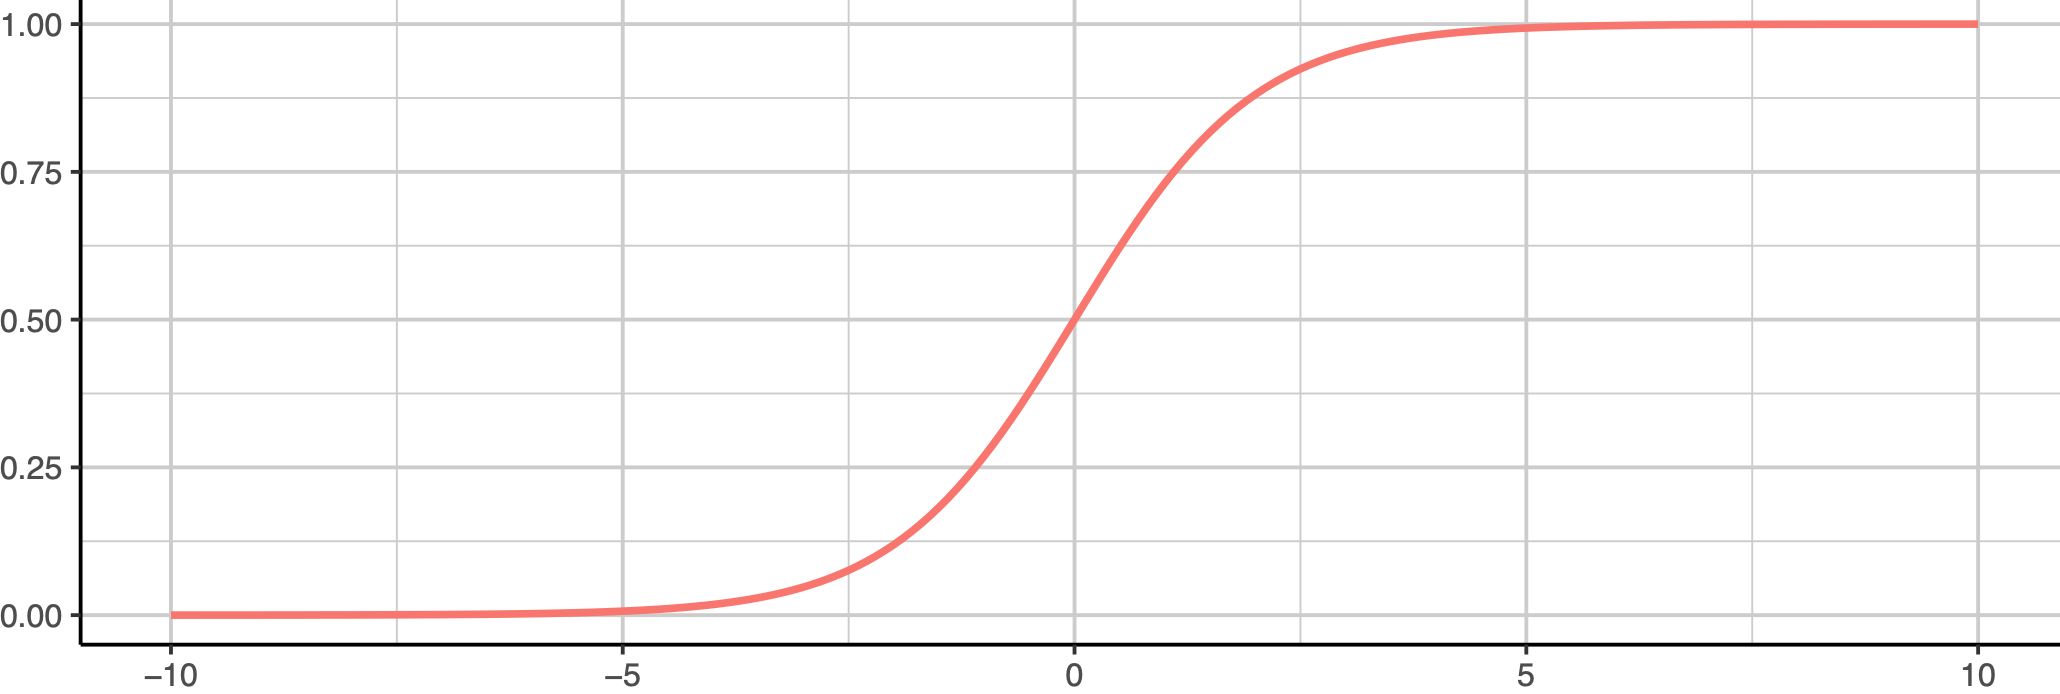
\includegraphics{plots/sigmoid.png}}
\end{figure}
\end{vbframe}
%%%%%%%%%%%%%%%%%%%%%%%%%%%%%%%%%%%%%%%%%%%%%%%%%%%%%%%%%%%%%%%%%%

\begin{vbframe}{Deep Feedforward Network}
  \lz
  \begin{figure}
    \centering
      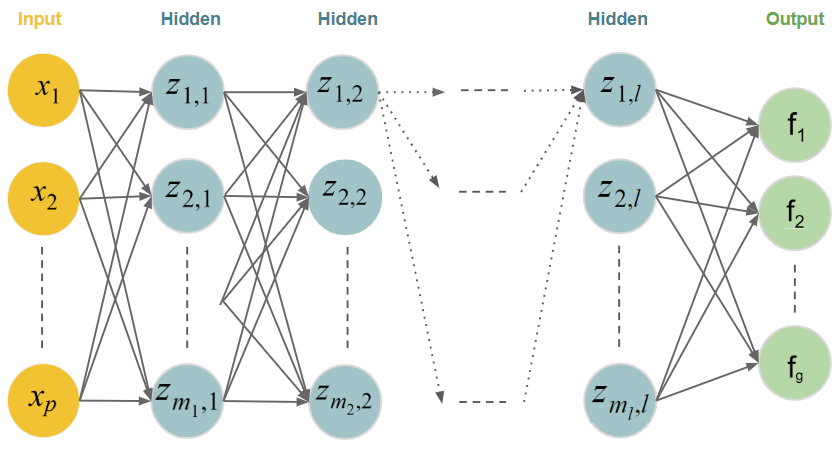
\includegraphics[width=10.5cm]{plots/deepneuralnet_new.png}
      \caption{Structure of a deep neural network with $l$ hidden layers.}
  \end{figure}
\end{vbframe}  

%%%%%%%%%%%%%%%%%%%%%%%%%%%%%%%%%%%%%%%%%%%%%%%%%%%%%%%%%%%%%%%%%%

\begin{vbframe}{Why add more layers?}
\begin{itemize}
\item Multiple layers allow for the extraction of more and more abstract
representations.
\lz
\item Each layer in a feed-forward neural network adds its own degree of non-linearity to the model.
\end{itemize}
\lz
\begin{figure}
\centering
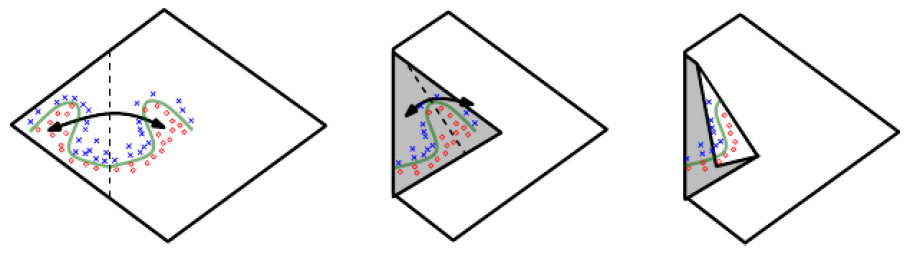
\includegraphics[width=10.5cm]{plots/folding}
\caption{An intuitive, geometric explanation of the exponential advantage of deeper networks formally (Mont\'{u}far et al. (2014)).}
\end{figure}
\end{vbframe}
%%%%%%%%%%%%%%%%%%%%%%%%%%%%%%%%%%%%%%%%%%%%%%%%%%%%%%%%%%%%%%%%%%

\begin{vbframe}{Deep neural networks}

Neural networks today can have dozens or even hundreds of hidden layers. The greater the number of layers, the "deeper" the network. Historically, however, deep neural networks were very challenging to train for several reasons:
\lz
\begin{enumerate}
\item For one thing, the use of sigmoid activations (e.g., logistic sigmoid and tanh) significantly slowed down training due to a phenomenon known as \enquote{vanishing gradients}. The introduction of the ReLU activation largely solved this problem.
\item Training deep neural networks on CPUs was too slow to be practical. Switching over to GPUs cut down training time by more than an order of magnitude.
\item Another reason neural networks were not popular until the late '00s is that when dataset sizes are small, other models (such as SVMs) and techniques (such as feature engineering) outperform them. 
\end{enumerate}
\framebreak
%%%%%%%%%%%%%%%%%%%%%%%%%%%%%%%%%%%%%%%%%%%%%%%%%%%%%%%%%%%%%%%%%%
\begin{itemize}
\item The availability of large datasets and novel architectures that are capable to handle even complex tensor-shaped data (e.g. CNNs for image data), faster hardware, and better optimization and regularization methods made it feasible to successfully implement deep neural networks in the last decade.
\lz

\item An increase in depth often translates to an increase in performance on a given task. State-of-the-art neural networks, however, are much more sophisticated than the simple architectures we have encountered so far.

\lz
\item The term "\textbf{deep learning}" encompasses all of these developments and refers to the field as a whole.
\end{itemize}
\end{vbframe}
%%%%%%%%%%%%%%%%%%%%%%%%%%%%%%%%%%%%%%%%%%%%%%%%%%%%%%%%%%%%%%%%%%

\endlecture
\end{document}
